\documentclass[a4paper]{article}
\addtolength{\hoffset}
{-2.25cm}
\addtolength{\textwidth}
{5cm}
\addtolength{\voffset}
{-3.25cm}
\addtolength{\textheight}
{5.5cm}
\setlength{\parskip}{0pt}
\setlength{\parindent}{0in}

\usepackage[utf8]{inputenc}
\usepackage{microtype}
\usepackage[english]{babel}
\usepackage{fancyhdr}
\usepackage{advdate}
\usepackage{enumitem}
\usepackage{amsmath, amssymb}
\usepackage{graphicx}
\usepackage{caption}
\usepackage{subcaption}
\usepackage{float}
\usepackage{titlesec}
\usepackage{wasysym}
\usepackage{url}
\usepackage{hyperref}
\usepackage{tikz, verbatimbox}
\usepackage{fixltx2e}
\usepackage{centernot}
\usepackage{algorithm}
\usepackage{algpseudocode}
\usepackage{listings}
\usetikzlibrary{shapes.geometric, arrows}
\usetikzlibrary{positioning}
\usepackage[table]{xcolor}

\graphicspath{{./static/}}
\tikzset{every picture/.style={line width=0.75pt}} %set default line width to 0.75pt

\newcommand{\LComment}[1]{\State \(\triangleright\) \text{#1}}
\MakeRobust{\Call}
\usepackage{pdfpages}

\newlength{\originalVOffset}
\newlength{\originalHOffset}
\setlength{\originalVOffset}{\voffset}   
\setlength{\originalHOffset}{\hoffset}

\begin{document}

\fancyhead[c]{}
\hrule \medskip
\begin{minipage}{0.295\textwidth}
\raggedright
Rishabh Indoria\\
21F3001823
\end{minipage}
\begin{minipage}{0.4\textwidth}
\centering
\LARGE
Programming Concepts using Java
\end{minipage}
\begin{minipage}{0.295\textwidth}
\raggedleft
\today \hfill \\
\end{minipage}
\medskip \hrule
\bigskip

\section{Introduction}
\subsection{Types}
\begin{itemize}
    \item \textbf{The role of types}: Interpreting data stored in binary consistently, i.e., viewing a sequence of bits as integers, floats, characters etc., Naming concepts and structuring out computations, Catching bugs early.
    \item \textbf{Dynamic Typing}: Derive type from the current value, $x=10$ means $x$ is of type $int$.
    \item \textbf{Static Typing}: Associate a type in advance with a name, $int$ $x$.
    \item In static typing $x$ will remain $int$ for its lifetime, i.e., cannot assign float or char value to $x$ whereas this is possible in dynamic typing.
    \textbf{Static analysis}: With variable declarations, compilers can detect type errors at compile time.
    \item Whereas dynamic typing would catch these errors only when the code runs.
    \item Compilers can also perform optimizations based on static analysis.
\end{itemize}

\subsection{Memory Management}
\begin{itemize}
    \item Variables store intermediate values during computation.
    \item Typically these values are local to a function but can also refer to global variables outside the function as well.
    \item \textbf{Scope} of a variable means when the variable is available to use.
    \item \textbf{Lifetime} of a variable is how long the storage remains allocated.
    \item "Hole in the scope": Variable is alive but not is scope.
    \item \textbf{Memory stack}: Each function needs storage for local variables. Create \textbf{an activation record} when function is called.
    \item Activation record are stacked which is popped when the function exits.
    \item \textbf{Control link} points to start of previous record.
    \item \textbf{Return value link} tells where to store the result.
    \item When a function is called, arguments are substituted for formal parameters.
    \item Parameters are part of the activation record of the function. Values are populated on function call. Like having implicit assignment statements at the start of the function.
    \item \textbf{Call by value}: Copy the value, updating the value inside the function has no side effect.
    \item \textbf{Call by reference}: parameter points to same location as the argument, updating the value will have side effects.
    \item Need a separate storage for persistent data, usually called the heap.
    \item Conceptually, allocate heap storage from "opposite" end with respect to the stack.
    \item Heap store outlives the activation record whereas in stack, variables are deallocated when a function exits.
    \item After deleting a node in a linked list, deleted node is now dead storage, unreachable, requires some memory management.
    \item \textbf{Manual Memory Management}: Programmer explicitly requests and returns heap storage. This is error-prone, memory leaks, invalid arguments.
    \item \textbf{Automatic Garbage Collection}: Run-time environment checks and cleans up dead storage. Marks all storage that is reachable from program variables and return all unmarked memory cells to free space. Convenience for programmer vs performance penalty.
    \begin{figure}[H]
        \centering
        \begin{subfigure}[b]{0.45\textwidth}
            \centering
            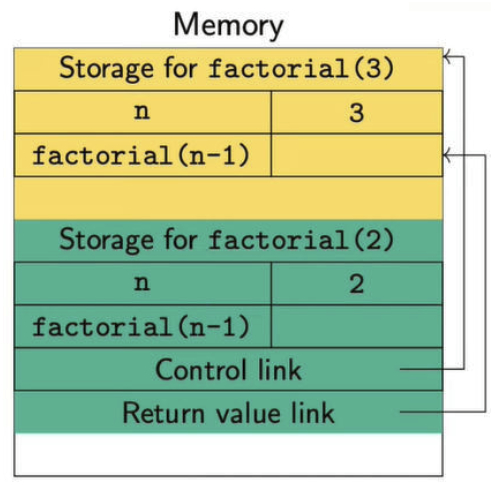
\includegraphics[width=\linewidth]{Diplomas//static/Java_activation_record.png}
            \caption{Activation Record Example}
            \label{fig:java-activation-record}
        \end{subfigure}
        \hfill
        \begin{subfigure}[b]{0.45\textwidth}
            \centering
            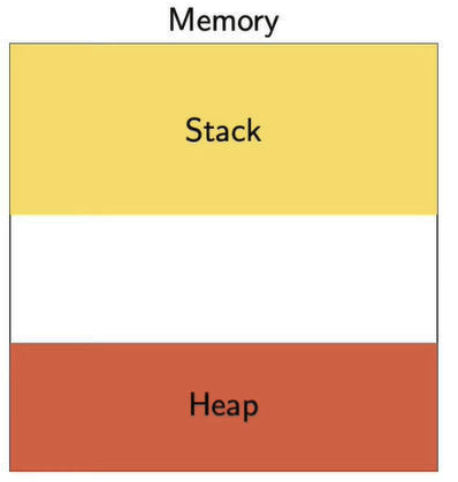
\includegraphics[width=\linewidth]{Diplomas/static/Java_heap.png}
            \caption{Heap Memory}
            \label{fig:java-heap-memory}
        \end{subfigure}
    \end{figure}
\end{itemize}

\subsection{Stepwise Refinement}
\begin{itemize}
    \item Begin with a high level description of the task.
    \item Refine the tasks into subtasks, and further elaborate each subtask.
    \item Subtasks can be coded by different people.
    \item \textbf{Program refinement}: focus on code, not much change in data structures.
\end{itemize}

\subsection{Modular Software Development}
\begin{itemize}
    \item Use refinement to divide the solution into components. Build a prototype of each component to validate design.
    \item Components are described in terms of interfaces and specification.
    \item \textbf{Interfaces}: What is visible to other components, typically function calls.
    \item \textbf{Specification}: Behavior of the component, as visible through the interface.
    \item Improve each component independently, preserving interface and specification.
\end{itemize}

\subsection{Programming Language support for Abstraction}
\begin{itemize}
    \item \textbf{Control Abstraction}: Functions and procedures. Encapsulate a block of code, reuse in different contexts.
    \item \textbf{Data Abstraction}: Abstract data types(ADT), set of values along with operations permitted on them. Internal representation should not be accessible, interaction should be restricted to public interface.
    \item \textbf{Object-Oriented Programming}: Organize ADTs in a hierarchy. Implicit reuse of implementations, subtyping, inheritance.
\end{itemize}

\section{Object-Oriented Programming}
\subsection{Classes and Objects}
\begin{itemize}
    \item An object is like an abstract data type. Hidden data with set of public operations.
    \item All interactions are done through operations.
    \item Uniform way of encapsulating different combinations of data and functionality.
    \item Classes are a template for a data type, i.e., how a data is stored and how public functions manipulate the data.
    \item Objects are concrete instances of the above mentioned template. Each object maintains its separate copy of local data. Invoking methods on objects is equivalent to "send a message to the object".
    \item Point example in python
    \begin{lstlisting}[language=Python]
        class Point:
            def __init__(self, a=0, b=0):
                self.x = a
                self.y = b
            def translate(self, dx, dy):
                self.x += dx
                self.y += dy
            def odistance(self):
                import math
                d = math.sqrt(self.x*self.x + self.y*self.y)
                return d
    \end{lstlisting}
    \item We can change the internal implementation from $(x,y)$ to $(r,\theta)$.
\end{itemize}

\subsection{Abstraction}
\begin{itemize}
    \item Objects are similar to abstract data types. They have public interface, private implementation, and changing the implementation should not affect interactions with the object.
    \item Data-centric view of programming, focus on what data we need to maintain and manipulate.
    \item Refining data representation is naturally tied to updating methods that operate on the data.
    \item Users of the code should not know whether $Point$ uses $(x,y)$ or $(r,\theta)$ implementation.
\end{itemize}

\subsection{Subtyping}
\begin{itemize}
    \item We can arrange types in a hierarchy.
    \item A subtype is a specialization of a type.
    \item If $A$ is a subtype of $B$, then wherever an object of type $B$ is needed, an object of type $A$ can be used.
    \item Every object of type $A$ is also an object of type $B$. Think of subsets, if $X\subseteq Y$, every $x\in X$ is also in $Y$.
    \item If $f()$ is a method in $B$ and $A$ is a subtype of $B$, every object of $A$ also supports $f()$, although implementation of $f()$ can be different in $A$.
\end{itemize}

\subsection{Dynamic lookup}
\begin{itemize}
    \item Whether a method can be invoked on an object is a static property, aka \textbf{type checking}.
    \item How the method acts is a dynamic property of how the object is implemented.
    \item Invoke the same operation, each object "knows" which function to invoke.
    \item Different from \textbf{overloading}.
    \item A variable $v$ of type $B$ can refer to an object of subtype $A$.
    \item Static type of $v$ is $B$, but method implementation depends on runtime type $A$.
\end{itemize}

\subsection{Inheritance}
\begin{itemize}
    \item Reuse of implementations.
    \item Usually one hierarchy of types to capture both subtyping and inheritance.
    \item $A$ can inherit from $B$ iff $A$ is a subtype of $B$.
    \item Philosophically, the two are different.
    \item  Subtyping is a relationship of interfaces whereas Inheritance is a relationship of implementations.
\end{itemize}

\section{Java}
\subsection{First Taste of Java}
\begin{itemize}
    \item Let's start with printing "hello world".
    \begin{lstlisting}[language=Java]
        public class helloworld{
            public static void main(String[] args){
                System.out.println("hello, world");
            }
        }
    \end{lstlisting}
    \item All code in Java lies within a class. No free floating functions.
    \item Modifier $public$ specifies visibility.
    \item For the code to start, it requires the $main$ function with the correct signature.
    \item $static$ makes it, so the function can be run independent of objects.
    \item $System$ is a public class, $out$ is a \textbf{stream} object defined in $System$. $println()$ is a method associated with streams.
    \item A Java program is a collection of classes. Each class is defined in a separate file with the same name, with extension $.java$.
    \item Java programs are usually interpreted on \textbf{Java Virtual Machine (JVM)}.
    \item $javac$ compiles into JVM \textbf{byte code}. $java$ runs the code.
    \item $javac$ should be provided $.java$ extension and $java$ should not be provided $.class$.
\end{itemize}

\subsection{Data Types}
\begin{itemize}
    \item Java has 8 primitive data types. Size of each is fixed by JVM independent of native architecture.
    \begin{figure}[H]
        \centering
        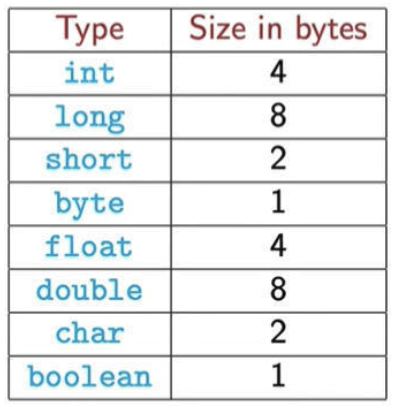
\includegraphics[width=0.5\linewidth]{Diplomas//static/Java_basic_types.png}
        \caption{Java Basic Data Types}
        \label{fig:Java-basic-types}
    \end{figure}
    \item We need to declare variables before we use them.
    \item Characters are written with \textbf{single-quotes}, strings are marked with \textbf{double-quotes}.
    \item Boolean constants are $true$, $false$.
    \item Modifier $final$ marks a constant. This variable cannot be updated later.
    \item Arithmetic operators are the usual ones $+,-,*,/,\%$
    \item When both arguments are integer, then $/$ is integer division.
    \item There is no exponentiation operator, use $Math.pow(a,n)=a^n$.
    \item $String$ is a built-in class. Strings are \textbf{not} an array of characters.
    \begin{lstlisting}[language=Java]
        String s = "Hello", t = "world";
        String u = s + " " + t; // "Hello world"
        s = s.substring(0,3) + "p!";
        int length = s.length();
    \end{lstlisting}
    \item If we change a $String$, we get a new object. $String$ are \textbf{immutable}.
    \item Arrays are also objects
    \begin{lstlisting}
        int[] a;
        a = new int[100];
        int[] b = new int[100];
        int length = a.length;
        a = {2, 3, 5, 7, 11};
    \end{lstlisting}
    \item In arrays, $length$ is a variable, whereas in strings $length()$ is a method. 
    \item Java allows limited \textbf{type inference} only for local variables in a function and not for instance variables in a function.
    \item Use generic $var$ to declare variables, these must be initialized when declared. Their type is inferred from initial value.
\end{itemize}

\subsection{Control Flow}
\begin{itemize}
    \item Start with conditional statements
    \begin{lstlisting}[language=Java]
        public class MyClass{
            ...
            public static int sign(int v){
            if (v < 0)
                return(-1);
            else if (v > 0)
                return(1);
            else
                return(0);
            }
        }
    \end{lstlisting}
    \item Conditional Loops
    \begin{lstlisting}[language=Java]
        public class MyClass{
            ...
            public static int sumupto(int n){
                int sum = 0;
                while (n > 0){
                    sum += n;
                    n--;
                }
                return(num);
            }
        }
    \end{lstlisting}
    \item Conditional loop can also be $do{...}while(c);$
    \item Iterative loop
    \begin{lstlisting}[language=Java]
        public class MyClass{
            ...
            public static int sumarray(int[] a){
                int sum = 0;
                int n = a.length;
                for(int i = 0; i < n; i++){
                    sum += a[i];
                }
                return(sum);
            }
        }
    \end{lstlisting}
    \item Java later introduced a $for$ in the style of Python
    \begin{lstlisting}[language=Java]
        for(type x : a){
            do something with x;
        }
    \end{lstlisting}
    \item Multiway branching aka switch case statement.
    \begin{lstlisting}[language=Java]
        public static void printsign(int v){
            switch(v){
                case -1:{
                    System.out.println("Negative");
                    break;
                }
                case 1:{
                    System.out.println("Positive");
                    break;
                }
                case 0:{
                    System.out.println("Zero");
                    break;
                }
                default:{
                    System.out.println("Fuck, Something went wrong");
                }
            }
        }
    \end{lstlisting}
\end{itemize}

\subsection{Defining Classes and Objects}
\begin{itemize}
    \item Definition block using $class$, with class name. Default visibility is public to $package$.
    \item All classes defined in the same directory from part of the same package.
    \item \textbf{Instance variable}: Each concrete object type $Date$ will have local copies of $date,month,year$. These are marked $private$. Can also have $public$ instance variable, but breaks encapsulation.
    \item Declare type using class name, $new$ creates a new object.
    \item $this$ is a reference to current object. We can omit $this$ is reference is unambiguous.
    \item We can add accessor and mutator methods to access and modify private variables.
    \item Constructors: Special functions called when an object is created. We can create multiple constructors with different signatures.
    \item A later constructor can call an earlier one using $this$ keyword.
    \item \textbf{Copy constructor} takes an object of the same type as an argument.
    \item If instance variables are objects, we may end up aliasing rather than copying aka shallow copy.
    \item An example of above concepts
    \begin{lstlisting}[language=Java]
        public class Date{
            private int day, month, year;
            public Date(int d, int m, int y){
                day = d;
                month = m;
                year = y;
            }
            public Date(int d, int m){
                this(d, m, 2021);
            }
            public Date(Date d){
                this.day = d.day;
                this.month = d.month;
                this.year = d.year;
            }
            public int getDay(){
                return(day);
            }
            public int getMonth(){
                return(month);
            }
            public int getYear(){
                return(year);
            }
        }

        public void useDate(){
            Date d1, d2;
            d1 = new Date(12, 4, 1954);
            d2 = new Date(d1);
        }
    \end{lstlisting}
\end{itemize}

\subsection{Input and Output}
\begin{itemize}
    \item We already saw an example of output.
    \item For input, the easiest to use is the $Console$ class, defined within $System$.
    \begin{lstlisting}[language=Java]
        Console cons = System.console();
        String username = cons.readLine("Username: ");
        char[] password = cons.readPassword("Password: ");
    \end{lstlisting}
    \item A more general $Scanner$ class, allows more granular reading of the input.
    \begin{lstlisting}[language=Java]
        Scanner in = new Scanner(System.in);
        String name = in.nextLine();
        int age = in.nextInt();
    \end{lstlisting}
    \item Output can be done with $System.out$.
    \item $println(arg)$ prints $arg$ and goes to a new line.
    \item $print(arg)$ prints $arg$ but doesn't advance to a new line.
    \item $printf(arg)$ generates formatted output, same convention as in $C$ language.
\end{itemize}

\subsection{Class Hierarchy}
\begin{itemize}
    \item Java does not allow multiple inheritance, it is tree like.
    \item In fact, there is a universal superclass $Object$.
    \item Few useful methods define in $Object$.
    \begin{lstlisting}[language=Java]
        public boolean equals(Object 0) // defaults to pointer equality
        public String toString() /* converts the value of 
        instance variables to String */
    \end{lstlisting}
    \item For Java object $x$ and $y$, $x==y$ invokes $x.equals(y)$
    \item Example of overriding $equals$ with $Date$
    \begin{lstlisting}[language=Java]
        public boolean equals(Object d){
            if(d instanceof Date){
                Date myd = (Date) d;
                return this.day == myd.day && this.month == myd.month &&
                this.year == myd.year;
            }
            return false;
        }
    \end{lstlisting}
    \item Overriding looks for "closest" match.
\end{itemize}

\subsection{Modifiers}
\begin{itemize}
    \item $public$ vs $private$ to support encapsulation of data.
    \item $static$, for entities defined inside classes that exist without creating objects of the class.
    \item $final$, for values that cannot be changed.
\end{itemize}

\subsection{Abstract Classes and Interfaces}
\begin{itemize}
    \item Provide an abstract definition of the method
    \begin{lstlisting}[language=Java]
        public abstract double perimeter();
    \end{lstlisting}
    \item Cannot create objects from a class that has abstract functions, and the class containing an abstract function must be declared abstract.
    \item Abstract class forces subclasses to provide a concrete implementations for abstract methods.
    \item We can still declare variable whose type is an abstract class.
    \item We can use abstract classes to specify generic properties.
    \begin{lstlisting}[language=Java]
        public abstract class Comparable{
            public abstract int cmp(Comparable s);
            // return -1 if this < s
            // return 0 if this == s
            // return 1 if this > s
        }
    \end{lstlisting}
    \item Now we can sort any array of objects that extend $Comparable$.
    \item An interface is an abstract class with no concrete components.
    \item An interface is an abstract class with no concrete components.
    \item We can extend only one class, but can implement multiple interfaces.
    \item Interface are basically classes with all methods being abstract.
    \begin{lstlisting}[language=Java]
        public interface Comparable{
            public abstract int cmp(Comparable s);
        }

        public class Circle extends Shape implements Comparable{
            public double perimeter(){...}
            public int cmp(Comparable s){...}
            ...
        }
    \end{lstlisting}
    \item Interface describes relevant aspects of a class. Abstract functions describe specific "slice" of capabilities.
    \item Java interfaces extended to allow functions to be added. We can provide a default implementation for some functions.
    \item If there is conflict between static/default methods then subclass must provide a fresh implementation.
    \item Conflict could be between a class and an interface, then the class "wins".
    \item \textbf{Functional interfaces}: Interfaces that define a single function. Examples can be Comparator, TimerOwner.
    \item We can use lambda expression to replace these
    \begin{lstlisting}[language=Java]
        Arrays.sort(strarr, (String s2, String s2) -> s1.length - s2.length)
    \end{lstlisting}
    \item More complicated function body can be defined as a block.
    \item We can reference static and instance methods as follows
    \begin{lstlisting}[language=Java]
        (x1, x2, ..., xk) -> f(x1, x2, ..., xk)
        (o, x1, x2, ..., xk) -> o.f(x1, x2, ..., xk)
    \end{lstlisting}
\end{itemize}

\subsection{Private Classes}
\begin{itemize}
    \item $LinkedList$ is built using $Node$. Why should $Node$ be public?
    \item Make $Node$ a private class nested within $LinkedList$, also called an \textbf{inner class}.
    \item Objects of private class can see private components of enclosing class.
\end{itemize}

\subsection{Controlled interaction with Objects}
\begin{itemize}
    \item Take the example of querying a database.
    \item Object stores train reservation information. We need to control spamming by bots, do this by requiring the user to login before querying.
    \item Need to connect the query to the logged in status of the user. Use objects, on login return a Query object.
    \item How does the user know the capabilities of the private object?, use an interface.
    \item Query object could allow unlimited number of queries. Limit the number of queries per login by maintaining a counter.
    \begin{lstlisting}[language=Java]
        public interface QIF{
            public abstract int getStatus(int trainno, Date d);
        }

        public class RailwayBooking{
            private BookingDB, railwayDB;
            public QIF login(String u, String p){
                QueryObject qobj;
                if(validLogin(u,p)){
                    qobj = new QueryObject();
                    return qobj;
                }
            }

            private class QueryObject implements QIF{
                private int numQueries;
                private final int QLIM;
                public int getStatus(int trainno, Date d){
                    if(numQueries < QLIM){
                        // Respond, increment numQueries
                    }
                }
            }
        }
    \end{lstlisting}
\end{itemize}

\subsection{Callbacks}
\begin{itemize}
    \item Myclass creates a Timer, and start it to run in parallel.
    \item Timer would notify Myclass when the time limit expires.
    \item Interface Runnable indicates that Timer can run in parallel.
    \begin{lstlisting}
        public interface TimerOwner{
            public abstract void timerDone();
        }

        public class MyClass implements TimerOwner{
            public void f(){
                ...
                Timer t = new Timer(this); // this object create t
                ...
                t.start(); // Start t
                ...
            }
            public void timerDone(){...}
        }

        public class Timer implements Runnable{
            // Timer can be invoked in parallel
            private TimerOwner owner;
            public Timer(TimerOwner o){
                owner = o; // Creator
            }
            public void start(){
                ...
                owner.timerDone();
            }
        }
    \end{lstlisting}
\end{itemize}

\subsection{Iterators}
\begin{itemize}
    \item We want to loop to run through all the values in a list, but we do not have public access, and we do not know which implementation it uses.
    \item Need the following abstraction
    \begin{lstlisting}[language=Java]
        Start at the beginning of the list
        while(there is a next element){
            get the next element;
            do something with it
        }
    \end{lstlisting}
    \item Create an $Iterator$ object and export it
    \begin{lstlisting}[language=Java]
        public interface Iterator{
            public abstract boolean has_next();
            public abstract Object get_next();
        }

        public class LinearList{
            private class Iter implements Iterator{
                private Node position;
                public Iter(){...}
                public boolean has_next(){...}
                public Object get_next(){...}
            }
            // Export a fresh iterator
            public Iterator get_iterator(){
                Iter it = new Iter();
                return it;
            }
        }
    \end{lstlisting}
    \item Definition of $Iter$ depends on the linear list.
    \item For nested loops. acquire multiple iterators.
\end{itemize}

\subsection{Generics Programming}
\begin{itemize}
    \item Use type variables. Type quantifier before return type.
    \item "For every type $T$ ..."
    \item Polymorphic $reverse$ in Java
    \begin{lstlisting}[language=Java]
        public <T> void reverse(T[] arr){
            T temp;
            int n = arr.length;
            for(int i = 0; i < n/2; i++){
                temp = arr[i];
                arr[i] = arr[(n - 1) - i];
                arr[(n - 1) - i] = temp;
            }
        }
    \end{lstlisting}
    \item The type parameter $T$ can also be applies to the class as a whole.
    \item We instantiate generic classes using concrete types.
    \begin{lstlisting}[language=Java]
        private class LinkedList<T>{
            public T head(){...}
            public void insert(T newdata){...}
        }

        LinkedList<Ticket> ticketList = new LinkedList<Ticket>();
    \end{lstlisting}
    \item Be careful not to accidentally hide a type variable
    \begin{lstlisting}[language=Java]
        public <T> void insert(T newDate){...}
    \end{lstlisting}
    \item $T$ in the argument of $insert()$ is a new $T$, different from the classes $T$.
    \item Java array typing is covariant, If $S$ extends $T$ then $S[]$ extends $T[]$.
    \item Generic classes are not covariant, $LinkedList<String>$ is not compatible with $LinkedList<Object>$.
    \item \textbf{Wildcards}: $?$ stands for an arbitrary unknown type. Avoids unnecessary type variable quantification when the type variable is not needed elsewhere.
    \begin{lstlisting}[language=Java]
        public static void printList(LinkedList<?> l){
            Object o;
            Iterator i = l.get_iterator();
            while(i.has_next()){
                o = i.get_next();
                System.out.println(o);
            }
        }
    \end{lstlisting}
    \item We can bound wild cards as follows
    \begin{lstlisting}[language=Java]
        public static void drawAll(LinkedList<? extends Shape>){...}
    \end{lstlisting}
    \item We can copy a linked list as follows
    \begin{lstlisting}[language=Java]
        public static <? extends T, T> void listcopy(LinkedList<?> src, LinkedList<T> tgt){...}
        public static <T, ? super T> void listcopy(LinkedList<T> src, LinkedList<?> tgt){...}
    \end{lstlisting}
\end{itemize}

\subsection{Reflection}
\begin{itemize}
    \item \textbf{Introspection}: A program can observe, and therefore reason about its own state.
    \item \textbf{Intercession}: A program can modify its execution state or alter its own interpretation or meaning.
    \item Suppose we want to write a function to check if two different objects are both instances of the same class?
    \begin{lstlisting}[language=Java]
        import java.lang.reflect;
        class MyReflectionClass{
            ...
            public static boolean classequal(Object o1, Object o2){
                return o1.getClass() == o2.getClass();
            }
        }
    \end{lstlisting}
    \item $getClass()$ returns an object of type $Class$ that encodes class information.
    \item For each currently loaded class $C$, Java creates an object of type $Class$ with information about $C$.
    \item We can create new instances of a class at runtime.
    \begin{lstlisting}[language=Java]
        Class c = obj.getClass();
        Object o = c.newInstance();
        String s = "Manager"'
        Class c = Class.forName(s);
        Object o = c.newInstance();
    \end{lstlisting}
    \item From the $Class$ object we can extract more data as well
    \begin{lstlisting}[language=Java]
        Class c = obj.getClass();
        Constructor[] constructors = c.getConstructors();
        Method[] methods = c.getMethods();
        Field[] fields = c.getFields();
    \end{lstlisting}
    \item These in turn have functions to get further details.
    \item We can also invoke methods and examine/set values of fields
    \begin{lstlisting}
        Class c = obj.getClass();
        Constructor[] constructors = c.getConstructors();
        Class params[] = constructors[0].getParameterTypes();
        Method[] methods = c.getMethods;
        Object[] args = {...};
        methods[3].invoke(obj, args); // invoke methods[3] on obj with argument args
        Field[] fields = c.getFields();
        Object o = fields[2].get(obj);
        fields[3].set(obj, value);
    \end{lstlisting}
    \item All of these only extract publicly defined values.
    \item For private use $getDeclaredConstructors()$, similar for rest.
    \item \textbf{BlueJ}, a programming environment to learn Java.
\end{itemize}

\subsection{Erasure of Generics}
\begin{itemize}
    \item \textbf{Type Erasure}: Java does not keep record of all versions of $LinkedList<T>$ as separate types. At run time, all type variables are promoted to $Object$ or an upper bound if one is available.
    \item $LinkedList<T>$ becomes $LinkedList<Object>$ and $LinkedList<?$ extends $Shape>$ becomes $LinkedList<Shape>$.
    \item So, we cannot use if(o instanceof T)
    \item As a consequence $LinkedList<Employee>$ and $LinkedList<Date>$ are the same class.
    \item Wrapper classes for basic types
    \begin{figure}[H]
        \centering
        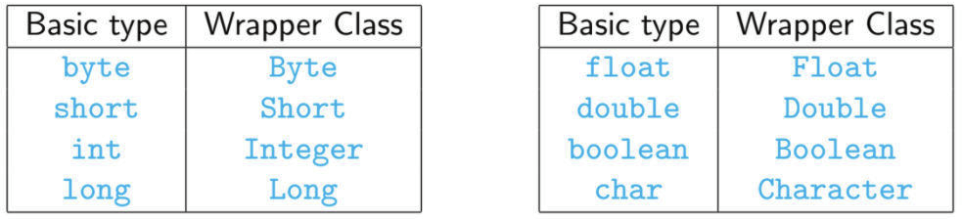
\includegraphics[width=0.6\linewidth]{Diplomas//static/Java_wrapper_class.png}
        \caption{Wrapper Class}
        \label{fig:Java-wrapper-class}
    \end{figure}
    \item All wrapper classes other than $Boolean$, $Character$ extend the class $Number$.
    \item Converting from basic type to wrapper class and back, there is also autoboxing, i.e., implicit conversion
    \begin{lstlisting}
        int x = 5;
        Integer myx = Integer(x);
        Integer myy = x;
        int y = myx.intValue();
        int x = myy;
    \end{lstlisting}
\end{itemize}

\subsection{Collections}
\begin{itemize}
    \item Most programming languages provide built-in collective data types, Arrays, Lists, Dictionaries.
    \item The $Collection$ interface abstracts properties of grouped data, $Arrays$, $Lists$, $Sets$, any non key-value structures.
    \item Two methods $add()$, that adds to the collection. $iterator()$, get an object that implements $Iterator$ interface.
    \item Iterator uses $hasNext()$ and $next()$ methods.
    \item Iterator also has $remove()$ method, removes the element that was last accessed by $next()$.
    \item The $Collection$ interface implements a lot of methods
    \begin{lstlisting}[language=Java]
        public interface Collection<E>{
            boolean add(E element);
            Iterator<E> iterator();
            int size();
            boolean isEmpty();
            boolean contains(Object obj);
            boolean containsAll(Collection<?> c);
            boolean equals(Object other);
            boolean addAll(Collection<? extends E> from);
            boolean remove(Object obj);
            boolean removeAll(Collection<?> c);
        }
    \end{lstlisting}
    \item $AbstractCollection$ class provides default implementation of the interface.
\end{itemize}

\subsection{Concrete Collections}
\begin{itemize}
    \item Interface $List$ for ordered collections.
    \item $ListIterator$ extends $Iterator$ and adds $add(E element)$, $previous()$, $hasPrevious()$ methods.
    \begin{lstlisting}[language=Java]
        public interface List<E> extends Collection<E>{
            void add(int index, E element);
            void remove(int index);
            E get(int index);
            E set(int index, E element);
        }
    \end{lstlisting}
    \item $AbstractList$ provides default implementation of $List$.
    \item Interface $Set$ for collection without duplicates, identical to $Collection$ but with constraints.
    \item $HashSet$ implements a hash table. It is unordered, but supports $iterator()$ that scans in unspecified order.
    \item $TreeSet$ uses a tree representation, values are ordered and maintains a sorted collection.
    \item Interface $Queue$ for ordered collections with constraints on addition and deletion.
    \item Can be $Dequeue$ or $PriorityQueue$.
\end{itemize}

\subsection{Maps}
\begin{itemize}
    \item Key value structures come under the $Map$ interface.
    \item Two type parameters, $K$ is for keys and $V$ is for values.
    \item $get(k)$ fetches the value for the key $k$, and $put(k, v)$ updates the value for the key $k$.
    \item $put(k,v)$ returns the previous value associated with $k$.
    \item Also implements $getOrDefault(k, v')$
    \item Also implements $putIfAbsent(key, 0)$
    \item We also have $keySet()$, $valueSet()$, and $entrySet()$.
    \item $HashMap$ works similar to $HashSet$, there is no fixed order.
    \item $TreeMap$ is similar to $TreeSet$, uses a balanced search tree to store. An iterator over $keySet()$ will process the keys in a sorted order.
    \item $LinkedHashMap$ remembers the order in which keys were inserted. Iterators will enumerate in the order of insertion. Similar to $LinkedHashSet$.
\end{itemize}

\subsection{Error Handling}
\begin{itemize}
    \item Code could encounter many types of errors, it should kill itself.
    \item Code that generates an error raises or throws an exception.
    \item Caller catches the exception and takes corrective action or pass the exception back up the calling chain.
    \item All exceptions descend from class $Throwable$ which has two branches $Error$ and $Exception$.
    \item $Error$ are relatively rare, "not the programmer's fault".
    \item $Exception$ has two sub-branches, one of which is $RunTimeException$.
    \item Enclose the code that may generate an exception in a $try$ block and the exception handler code should be in $catch$ block.
    \begin{lstlisting}[language=Java]
        try{
            call a function that may throw an exception
        } catch(ExceptionType e){
            examine e and handle it
        }
    \end{lstlisting}
    \item Can catch more than one exception, catch blocks are tried sequentially.
    \item Order $catch$ blocks by argument type, more specific to less specific.
    \item We can also $throw$ a checked exception.
    \item Example: throw new EOFException(errormsg);
    \begin{lstlisting}[language=Java]
        String readData(Scanner in) throws EOFException{
            ...
            while(...){
                if(n < len){
                    throw new EOFException(errmsg);
                }
            }
        }
    \end{lstlisting}
    \item Can throw multiple types of exception. Can throw subtype of declared exception type.
    \item If we call such a method, we must handle it or pass it on.
    \item Can also create custom exception
    \begin{lstlisting}[language=Java]
        public class NegativeException extends Exception{
            private int error_value;
            // Negative value that generated exception
            public NegativeException(String message, int i){
                super(message); // Appeal to the super class
                error_value = i; // Constructor to set message
            }
            public int report_error_value(){
                return error_value;
            }
        }
    \end{lstlisting}
    \item We can extract information about the exception $e.getMessage()$, $getCause()$, $initCause()$.
    \item When an exception occurs, rest of the $try$ block is skipped. We may need to do some clean up, add a block labelled $finally$.
\end{itemize}

\subsection{Packages}
\begin{itemize}
    \item Java has an organizational unit called $package$.
    \item Can use $import$ to use packages directly, $import\text{ }java.math.BigDecimal$
    \item Get all classes as $import\text{ }java.math.*$, $*$ is not recursive.
    \item We can declare packages as $package\text{ }in.ac.iitm.onlinedegree$. Name is based on folder hierarchy, with $in$ being the root folder.
    \item $protected$ means visible within the subtree, so all subclasses. $protected$ can be made $public$.
\end{itemize}

\subsection{Assertions}
\begin{itemize}
    \item Functions may have constraints on the parameters, we "assert" the property we assume to hold.
    \begin{lstlisting}[language=Java]
        public static double myfn(double x){
            assert x >= 0 : x;
        }
    \end{lstlisting}
    \item If assertion fails, the code will throw $AssertionEror$, this should not be caught. Colon provides additional information to be printed with the diagnostic message.
    \item Assertions are enabled or disabled at runtime, does not require re-compilation.
    \item $java\text{ }-enableassertions\text{ }MyCode$, or we could use $-ea$.
    \item Can also selectively enable assertions as $java\text{ }-ea:Myclass\text{ }MyCode$
    \item Similar for disable assertions, $-da$.
    \item To enable assertions for system class, use $-esa$ or enable system assertions.
\end{itemize}

\subsection{Logging}
\begin{itemize}
    \item It is rather typical to generate messages within code for diagnosis. Naive approach is to use the print statements.
    \item Instead log diagnostic messages separately, logs are arranged hierarchically.
    \item Simplest info call
    \begin{lstlisting}[language=Java]
        Logger.getGlobal().info("Edit->Copy menu item selected");
    \end{lstlisting}
    \item We can suppress logging by executing
    \begin{lstlisting}[language=Java]
        Logging.getGlobal().setLevel(Level.OFF);
    \end{lstlisting}
    \item Can also create custom logger
    \begin{lstlisting}[language=Java]
private static final Logger myLogger = Logger.getLogger("in.ac.iitm.onlinedegree");
    \end{lstlisting}
    \item Logger names are hierarchical, like package names.
    \item There are seven logging level, SEVERE, WARNING, INFO, CONFIG, FINE, FINER, FINEST.
    \item By default, first three levels are logged
    \item We can set a different level
    \begin{lstlisting}[language=Java]
        logger.setLevel(Level.FINE);
    \end{lstlisting}
    \item Turn on or off all logging using Level.ALL and Level.OFF.
\end{itemize}

\subsection{Cloning}
\begin{itemize}
    \item Normal assignment creates two references to the same object. Basically, two different variables point to the same object in memory.
    \item Object defines a method $clone()$ that returns a bitwise copy.
    \item If the object that is being copied has an array then only the pointer is copied, so bitwise copy is \textbf{shallow copy}.
    \item For \textbf{deep copy} we can override the $clone()$ method, first call $super$ then replace all arrays with fresh copies.
    \item To allow $clone()$, class must implement $Cloneable$ interface.
    \item $clone()$ in Object is protected, redefine it to be public.
    \item $clone()$ in Object throws CloneNotSupportedException which must be taken into account when overriding.
\end{itemize}

\subsection{Streams}
\begin{itemize}
    \item Suppose we have split a text file as a list of words, we generate a stream of values from a collection.
    \item Operations transform input streams to output streams.
    \begin{lstlisting}[language=Java]
        List<String> words = ...;
        long count = words.stream().filter(w -> w.length() > 10).count();
    \end{lstlisting}
    \item Stream processing is declarative, and processing can be parallelized parallelStream().
    \item Lazy evaluation is possible.
    \item A stream does not store its elements.
    \item Stream operations are non-destructive, input stream is untouched.
    \item We create a stream, transform it and then reduce it to a result.
    \item Apply $stream()$ to a collection. Use static method $Stream.of()$ for arrays.
    \item $Stram.generate()$ generates a stream from a function and $Stream.iterate()$ is a stream of dependent values.
    \begin{lstlisting}[language=Java]
        Stream<String> randomds = Stram.generate(Math::random);
        Stream<Integer> integers = Stream.iterate(0, n -> n < 100, n -> n + 1);
    \end{lstlisting}
    \item $filter()$ to select elements, takes a predicate as arguments.
    \item $map()$ applies a function to each element in the stream.
    \item If $map()$ function generates a list, we can instead use $flatMap()$ to flatten the list.
    \item $limit(n)$, makes a stream finite.
    \item $skip(n)$, skips first $n$ elements.
    \item $takeWhile()$, stop when element matches a criterion.
    \begin{lstlisting}[language=Java]
        Stream<Double> randomds = Stream.generate(Math::random).takeWhile(n -> n >= 0.5)
    \end{lstlisting}
    \item $dropWhile()$, start after element matches a criterion.
    \item $count()$, count the number of elements.
    \item $max()$ and $min()$, requires a comparison function.
    \item $findFirst()$, returns the first element.
    \item If the stream is empty then the termination functions will return null or no object.
    \item We can use $orElse()$, $orElseGet()$, $orElseThrow()$
    \begin{lstlisting}[language=Java]
        Double fixrand = maxrand.orElse(-1.0);
    \end{lstlisting}
    \item We can also ignore missing values $ifPresent(v -> Process v)$, or $isPresentOrElse$
    \item We can create an optional value, $Optional.of(v)$ or $Optional.empty()$. Can also use $Optional.ofNullable()$ to transform $null$ into an empty optional.
    \item We can produce an output $Optional$ value from an input $Optional$.
    \item Can convert a stream into an array using $toArray()$.
    \item Can use $collect(Collectors.toList())$ to convert stream back into a collection. It can be any collection, doesn't have to be list.
    \item $summarizingInt$ works for a stream of integers that stores count, max, min, sum, average. Can be accessed using $getCount()$.
    \item We can convert stream to map as well, similar syntax, requires what key and value to take. Can store entire object as value using $Function.identity()$.
    \item We can read and write raw bytes using $InputStream$ and $OutputStream$.
    \item Use $in.available()$ to check if input is available, and $in.read(data)$ to read data and $in.close()$ to close the stream.
    \item Use $out.write(values)$ to write values to the output, and $out.flush()$ to flush the output, output is buffered.
    \item We can also connect to file using $FileInputStream(file)$ and $FileOutputStream(file, boolean)$. Boolean decides whether we are overwriting(false) or appending(true).
    \item Use $Scanner$ class as new Scanner(fin), where fin is $FileInputStream$.
    \item To write text use $PrintWriter$ class, has methods $println$ and $print$.
    \item To write binary data, use $DataOutputStream$ class.
    \item Fucking java has a zoo of streams.
\end{itemize}

\section{Philosophy of OOPs}
\subsection{Introduction}
\begin{itemize}
    \item Traditionally, algorithm comes first, and data representation comes later.
    \item OOPs reverses this focus.
    \item We design objects with few key points in mind.
    \item \textbf{Behavior}: What methods do we need to operate on objects?
    \item \textbf{State}: How does the object react when methods are invoked?
    \item \textbf{Encapsulation}: Should not change unless a method operates on it.
    \item \textbf{Identity}: Distinguish between different objects of the same class. State may be the same.
    \item Robust design minimizes dependencies, or coupling between classes.
\end{itemize}

\subsection{Subclasses and Inheritance}
\begin{itemize}
    \item A typical Java class
    \begin{lstlisting}[language=Java]
        public class Employee{
            private String name;
            private double salary;

            /* Constructors... */

            // Mutator methods
            public boolean setName(String s){...}
            public boolean set Salary(double x){...}

            // Accessor methods
            public String getName(){...}
            public int getSalary(){...}

            // Other methods
            public double bonus(float percent){
                return (percent/100.0) * salary'
            }
        }
    \end{lstlisting}
    \item Managers are special types of employees with extra features.
    \item $Manager$ object inherits other fields and methods from $Employee$. $Manager$ is a \textit{subclass} of $Employee$.
    \item $Manager$ objects do not automatically have access to private data of the parent class.
    \item Use parent class's constructor using $super$.
    \begin{lstlisting}[language=Java]
        public class Manager extends Employee{
            ...
            public Manager(String n, double s, String sn){
                super(n,s);
                secretary = sn;
            }
        }
    \end{lstlisting}
    \item In general, subclass has more features than parent class.
    \item Every $Manager$ is an $Employee$, but every $Employee$ is not a $Manager$.
    \begin{lstlisting}[language=Java]
        Employee e = new Manager(...);
    \end{lstlisting}
    \item The above works, but reverse does not.
\end{itemize}

\subsection{Dynamic dispatch and Polymorphism}
\begin{itemize}
    \item $Manager$ can redefine $bonus()$. Use parent class $bonus$ via $super.bonus()$.
    \item Consider the following assignment
    \begin{lstlisting}
        Employee e = new Manager(...);
    \end{lstlisting}
    \item $e$ can only refer to methods in $Employee$.
    \item If a method is defined in both $Employee$ and $Manager$, then $e$ will consider method defined in $Manager$, this is \textbf{dynamic dispatch}.
    \item Signature of a function is its name and the list of argument types.
    \item Can have different functions with the same name and different signatures.
    \item Java class $Arrays$ has a method $sort$ to sort arbitrary scalar arrays.
    \item \textbf{Overloading}: multiple methods, same name, different signature(different parameters), choice is static.
    \item \textbf{Overriding}: multiple methods, same name, same signature, choice is static.
    \item \textbf{Dynamic Dispatch}: multiple methods, same signature, choice made at run-time.
    \item Consider the method $getSecretary()$, which is only defined in $Manager$ class.
    \item The earlier definition of $e$ cannot invoke this method directly, instead we need \textbf{type casting}.
    \begin{lstlisting}[language=Java]
        ((Manager) e).getSecretary();
    \end{lstlisting}
    \item Cast fails at run time if $e$ is not a $Manager$.
    \item We can test if $e$ is $Manager$ as
    \begin{lstlisting}[language=Java]
        if(e instanceof Manager){
            ((Manager) e).getSecretary();
        }
    \end{lstlisting}
    \item We can also use type casting for basic data types.
\end{itemize}

\subsection{Benefits of Indirection}
\begin{itemize}
    \item To use different implementation of $Queue$ or any other data structure.
    \begin{lstlisting}[language=Java]
        Queue<Date> dateq;
        Queue<String> stringq;
        dateq = new CircularArrayQueue<Date>();
        stringq = new LinkedListQueue<String>();
    \end{lstlisting}
\end{itemize}

\section{Concurrent Programming}
\subsection{Threads and Processes}
\begin{itemize}
    \item Multiprocessing, single processor executes several computations "in parallel".
    \item It's basically switching between different actions very fast.
    \item Have a class extend $Thread$ and define a function $run()$ where execution can begin in parallel.
    \item Invoking $start$ on the object will start $run$ in a separate thread.
    \begin{lstlisting}[language=Java]
        public class Parallel extends Thread{
            private int id;
            public Parallel(int i){id = i;}
            public void run(){
                for(int j = 0; j < 100; j++){
                    System.out.println("id: " + id);
                }
                try{
                    // Sleep for 1000ms
                    sleep(1000);
                }catch(InterruptedException e){...}
            }
        }
    \end{lstlisting}
    \item Directly calling $run$ will also execute in a separate thread.
    \item Since, we cannot always extend $Thread$ we instead implement $Runnable$.
    \item To use $Runnable$, we need to explicitly create a $Thread$ object and invoke $start$ on the object.
\end{itemize}

\subsection{Race Conditions}
\begin{itemize}
    \item \textbf{Race Condition}: Concurrent update of shared variables, unpredictable outcome.
    \item Mutually exclusive access to critical regions of code, make sure two threads don't access the shared variable at once.
    \item We can try to do this by introducing another shared variable $turn$, that decides which thread has access. The problem with this, if one thread shuts down randomly, then others are locked out permanently leading to \textbf{Starvation}.
    \item Another approach can be as follows, but this can lead to \textbf{Deadlock}, where both threads try simultaneously.
    \begin{figure}[H]
        \centering
        \begin{subfigure}[b]{0.45\textwidth}
            \centering
            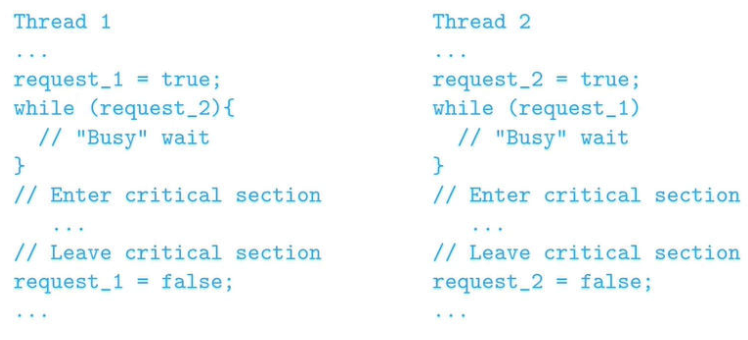
\includegraphics[width=\linewidth]{Diplomas//static/Java_deadlock.png}
            \caption{Deadlock}
            \label{fig:Java-deadlock}    
        \end{subfigure}
        \hfill
        \begin{subfigure}[b]{0.45\textwidth}
            \centering
            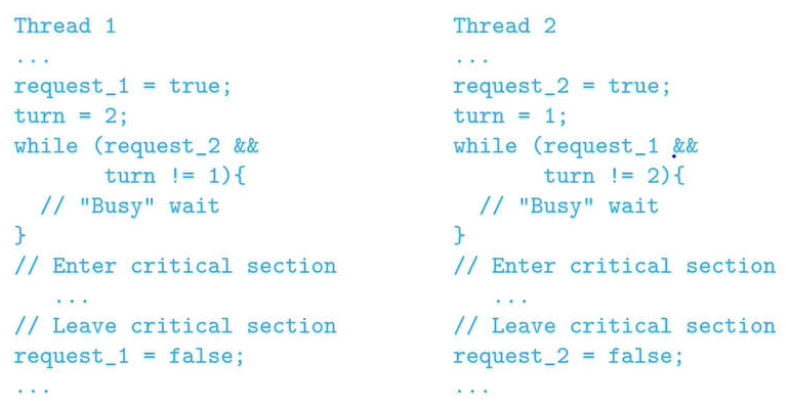
\includegraphics[width=\linewidth]{Diplomas/static/Java_Peterson_algorithm.png}
            \caption{Peterson's Algorithm}
            \label{fig:Java-peterson-alg}
        \end{subfigure}
    \end{figure}
    \item We can combine the previous two approaches into \textbf{Peterson's algorithm}.
    \item Generalizing this to more than two processes is not trivial.
    \item \textbf{Lamport's Bakery Algorithm}: Each new process picks p a token(increments a counter) that is larger than all waiting processes, the lowest token number gets served next, we still need to break ties.
\end{itemize}

\subsection{Semaphores}
\begin{itemize}
    \item The fundamental issue preventing consistent concurrent updates of shared variables is $test-and-set$.
    \item To increment a counter, check its current value, then add 1. If more than one thread does this in parallel, updates may overlap and get lost.
    \item Need to combine test and set into an atomic, indivisible step.
    \item Semaphores are a programming language's support for mutual exclusion.
    \item A semaphore $s$ supports two atomic operations
    \item $P(s)$: from Dutch \textit{passeren}, to pass.
    \item $V(s)$: from Dutch \textit{vrygeven}, to release.
    \begin{figure}[H]
        \centering
        \begin{subfigure}[b]{0.45\textwidth}
            \centering
            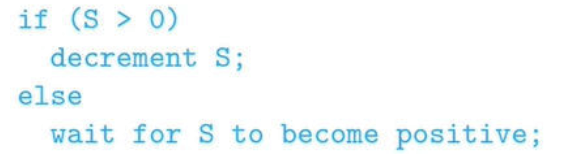
\includegraphics[width=\textwidth]{Diplomas/static/Java_P_s.png}
            \caption{P(s) automatically executes this}
            \label{fig:Java-P-s}
        \end{subfigure}
        \hfill
        \begin{subfigure}[b]{0.45\textwidth}
            \centering
            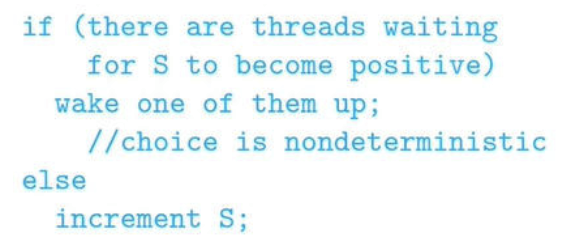
\includegraphics[width=\textwidth]{Diplomas/static/Java_V_s.png}
            \caption{V(s) automatically executes this}
            \label{fig:Java-V-s}
        \end{subfigure}
    \end{figure}
    \item Semaphores guarantee mutual exclusion, freedom from starvation and deadlock.
    \item However, they are too low level, and there is no clear relationship between a semaphore and the critical region that it protects.
\end{itemize}

\subsection{Monitors}
\begin{itemize}
    \item Attach synchronization control to the data that is being protected.
    \item Monitors are like a class, variables are the data that needs to be protected and functions are the ones that modify this data.
    \item Monitor guarantees mutual exclusion, if one function is active, any other function will have to wait for it to finish.
    \item $wait()$, all other processes are blocked out while this process waits.
    \item $notify()$, signals and exits.
    \begin{lstlisting}
        monitor bank_account{
            double accounts[100];
            queue q[100]; // one internal queue for each account
            boolean transfer(double amount, int source, int target){
                while(accounts[source] < amount){
                    q[source].wait(); // wait in the queue associated with source
                }
                accounts[source] -= amount;
                accounts[target] += amount;
                q[target].notify(); // notify the queue associated with target
                return true;
            }
        }
    \end{lstlisting}
    \item In java, this is written as
    \begin{lstlisting}[language=Java]
        public class bank_account{
            double accounts[100];
            public synchronized boolean transfer(double amount, int source, int target){
                while(accounts[source] < amount){wait();}
                accounts[source] -= amount;
                accounts[target] += amount;
                notifyAll();
                return true;
            }
            public synchronized double audit(){
                double balance = 0.0;
                for(int i = 0; i < 100; i++){
                    balance += accounts[i]
                }
                return balance;
            }
            public double current_balance(int i){
                return accounts[i]; // not synchronized
            }
        }
    \end{lstlisting}
    \item Rest of this is much easier to learn by practicing, there is no point in having notes for code.
\end{itemize}

\section{Graphical User Interfaces}
This is just easier to look up tutorials or projects to understand. Use the Swing Toolkit. Not that hard to use, checkout my \href{https://github.com/Risdorn/Mystery-Maze-Gameathon}{game} I made using it, it has no sound and is very buggy, but it works.

\end{document}